% Copyright 2023 Russell Goyder. All rights reserved.

\documentclass[12pt]{article}

\usepackage{graphicx}
\usepackage{hyperref}

\newcommand{\eg}{\emph{e.g.,}}
\newcommand{\Order}{\ensuremath{\mathcal{O}}}
\newcommand{\nn}{\nonumber}
\newcommand{\et}[1]{e^{\mbox{\small $#1$}}}
\newcommand{\lra}{\leftrightarrow}
\newcommand{\dt}{\! \cdot \!}
\newcommand{\wdg}{\! \wedge \!}
\newcommand{\crs}{\! \times \!}
\newcommand{\half}{{\textstyle \frac{1}{2}}}
\newcommand{\sig}{\sigma}
\newcommand{\gam}{\gamma}
\newcommand{\del}{\delta}
\newcommand{\Del}{\Delta}
\newcommand{\eps}{\epsilon}
\newcommand{\la}{\langle}
\newcommand{\ra}{\rangle}
\newcommand{\deriv}[2]{\frac{\partial #1}{\partial #2}}
\newcommand{\sigr}{\sig_r}
\newcommand{\sigth}{\sig_\theta}
\newcommand{\sigph}{\sig_\phi}
\newcommand{\dr}{\partial_r}
\newcommand{\rev}[1]{\tilde{ #1 }}
\newcommand{\om}{\omega}
\newcommand{\omy}{\omega_y}
\newcommand{\omd}{\omega_d}
\newcommand{\omsd}{\omega_{sd}}
\newcommand{\what}{\hat{w}}

\begin{document}

\title{The sundial problem from a new angle}
\author{Russell Goyder\footnote{Email: \texttt{russell.goyder@gmail.com}}}
\date{6th January 2024\footnote{Originally published in the \href{https://iopscience.iop.org/article/10.1088/0143-0807/27/2/023}{European Journal of Physics in 2006}}}
\maketitle

\begin{abstract}
  I present the age-old mathematics of the sundial from a new perspective. Standard approaches consider the problem in the Earth frame and focus on spherical geometry. In this work, I apply a more physical approach, based on geometric algebra, to the generalized sundial problem of calculating the position of the tip of the shadow of a gnomon on a flat dial surface, both of which can have arbitrary orientation. This results in exact parametric expressions for the analemma and equation of time, which reduce to standard results for the special cases of common dial types.
\end{abstract}

% ----------------------------------------------------------------- %
\section{Introduction}
%
Sundials are among the most ancient of mankind's inventions and the mathematics that describes them has been well understood for many centuries. A sundial consists of a shadow-casting object, called a gnomon\footnote{Traditionally, the word gnomon has been used to describe a vertical shadow-casting object but here we use it for one of arbitrary orientation.}, and a dial face displaying lines parallel to the shadow at different times of day. The problem considered here is to calculate the location of those lines. The common approach to solving this problem works relative to a frame fixed with respect to the Earth and the sun's apparent motion is parametrized via its hour angle which is zero at noon and increases by approximately $1^\circ$ every four minutes.

This has the advantage of decoupling the issue of dial geometry from the orbital dynamics of the Earth and sun; it removes the physics of orbits from the problem and reduces it to one of mathematics only. The physics is a part of the problem however, embodied in the ``equation of time'' and a full treatment must include it. Normally, it is presented somewhat separately (if at all), set apart from the geometry as viewed in the Earth's frame of reference.

In this paper, I apply a different approach to the calculation; one where both the orbital dynamics and the geometry of the dial are included in a single framework, based on the rest frame of the fixed stars. This yields expressions for both the equation of time and the coordinates of the tip of the shadow as it moves across the face of the sundial. I consider a geometry that is more general than that commonly considered in the literature; one where the orientation of both the gnomon and the dial face can be arbitrary.

This more general approach is facilitated by neat handling of rotations and other geometric operations afforded by geometric algebra. In fact, I was not aware that it was more general when first applying it; it was simply a natural way to tackle the problem, given the tools of geometric algebra. An introduction to these techniques is beyond the scope of this work. There are many excellent tutorials available\footnote{I would recommend starting at \href{http://geometry.mrao.cam.ac.uk/home/introduction-to-ga/}{http://geometry.mrao.cam.ac.uk}.}, such as \cite{inanr}, \cite{umlfpae} and \cite{GAbook}. This problem forms an instructive example of the application of rotors in particular, and of some simple techniques in geometric algebra in general.

We start in Section~\ref{secDefinitions} by defining some orthonormal frames, planes and other vectors which specify the geometry of the dial, its location on the Earth and the position of the Earth relative to the sun. We then write down the solution to the sundial problem in general terms in Section~\ref{mainCalc}. In Section~\ref{specCalc} we specialize to the case of a gnomon in the meridian plane and derive explicit forms of the general results of Section~\ref{mainCalc}, including an exact expression for the equation of time which is shown in Section~\ref{eot}. In Section~\ref{secPaths} we graph some example paths followed by the shadow tip as it moves across the dial face and Section~\ref{secComparison} contains a comparison of the results found in this work with standard formulae in the literature. Finally, we conclude in Section~\ref{secConclusion} and \ref{kepler} contains details of the novel approach taken to the Kepler problem, based on spinors and of which full details can be found in \cite{GAbook}.
%
% ----------------------------------------------------------------- %
\section{Definitions} \label{secDefinitions}
%
\subsection{Useful frames}
%
We begin with an orthonormal frame fixed relative to the the``fixed stars'' $\{e_i:i=1,2,3\}$ oriented as in Figure~\ref{universe_frame} such that $e_1$ is directed from the sun's centre of mass to that of the Earth at the summer solstice and $-e_2$ does the same at the vernal equinox. 
%
\begin{figure}[ht!]
\centering
\includegraphics[width=13cm]{figs/figure1.eps} 
\caption{The Earth's orbit around the sun and orientation of its axis of rotation. The orbit lies in the $e_1 \wdg e_2$ plane and the Earth's axis is $f_3$. The equinoxes and solstices lie on the points of intersection of the ellipse and the $\{e_i\}$ frame. Note that the axes of the ellipse are not aligned with $e_1$ and $e_2$ but differ by an angle $\rho$ which for the Earth is about $12.25^\circ$ and that the eccentricity of the Earth's orbit is greatly exaggerated.\label{universe_frame}}
\end{figure}
%
The origin of this frame's coordinate system is located at the focus of the Earth-sun orbit (their common centre of mass) and we consider these two bodies in isolation, ignoring the gravitational effect of other masses in the solar system. We can then define a frame fixed in the Earth by modelling its orientation as arising from two rotations; one in the $e_1 \wdg e_3$ plane by $\alpha$, the tilt of the Earth's axis and another in the Earth's equator by $\psi$, the rate at which the Earth spins relative to the fixed stars,
%
\begin{eqnarray}\label{fFrameRotors}
R_\alpha & = & \exp(-e_1 e_3\half\alpha) \\ \nn
R_\psi & = & \exp(-R_\alpha e_1 \rev{R}_\alpha e_2\half\psi).
\end{eqnarray}
%
Applying the rotor $R_\psi R_\alpha$ to the fixed $\{e_i\}$ frame gives
%
\begin{eqnarray}
f_1 & = & \phantom{-}\cos\psi( \cos\alpha \,e_1 + \sin\alpha \,e_3 ) + \sin\psi \,e_2\\ \nn
f_2 & = & - \sin\psi( \cos\alpha \,e_1 + \sin\alpha \,e_3 ) + \cos\psi \,e_2\\ \nn
f_3 & = & -\sin\alpha \,e_1 + \cos\alpha \,e_3.
\end{eqnarray}
%
$f_3$ is parallel to the Earth's axis of rotation and $f_1 \wdg f_2$ is the equatorial plane. Although $f_1$ and $f_2$ vary with time via $\psi$, the equatorial plane does not; the $\psi$ dependence cancels to give
%
\begin{equation}
 f_1 \wdg f_2 = \cos\alpha \; e_1 \wdg e_2 - \sin\alpha \; e_2 \wdg e_3.
\end{equation}
%
In Figure~\ref{universe_frame} this frame is shown at the summer solstice when $f_2$ is parallel to $e_2$. In this work we assume $\alpha$ is constant, but this is not quite the case; it varies by about $3^\circ$ with a period of $\sim41000$ years. We could include this effect in the current treatment by simply allowing $\alpha$ to vary with time. In addition, the earth's axis precesses with a period of $\sim23000$ years. Again, this effect is ignored in the current work but could be included by using another rotor in (\ref{fFrameRotors}).

To obtain the coordinate frame of an observer on the Earth's surface, we require a further rotation to account for latitude. Let us define $\theta$ as in Figure~\ref{fig:nframe}
%
\begin{figure}
\centering
\includegraphics[width=7cm]{figs/figure2.eps}
\caption{The orthonormal frame $\{n_i : i = 1,2,3\}$ on the Earth's surface, obtained by rotating the Earth frame $\{f_i\}$ by $\theta$ in the plane $f_3 \wdg f_1$. $n_3$ points vertically upward, toward the zenith. $n_1$ is directed South and $n_2$ East.\label{fig:nframe}}
\end{figure}
%
such that it matches the angle commonly denoted $\theta$ in the spherical polar coordinate system. The corresponding latitude $\theta_L = \pi/2 - \theta$. A rotation of $\theta$ in the $f_3 \wdg f_1$ plane
%
\begin{equation}
R_\theta = \exp(-f_3 \wdg f_1\half\theta)
\end{equation}
%
applied to the $\{f_i\}$ frame then gives us the orthonormal frame of an observer on the Earth's surface $\{n_i\}$
%
\begin{eqnarray} \label{nFrame}
n_1 & = & \left( \sin\alpha\sin\theta+\cos\alpha\cos\psi\cos\theta\ \right) \, e_1
		+ \sin\psi\cos\theta\,e_2 \\ \nn
	& & + \left( -\cos\alpha\sin\theta+\sin\alpha\cos\theta\cos\psi \right) \, e_3 \\ \nn
n_2 & = & - \sin\psi( \cos\alpha \,e_1 + \sin\alpha \,e_3 ) + \cos\psi \,e_2 \\ \nn
n_3 & = & \left( \cos\psi\cos\alpha\sin\theta-\sin\alpha\cos\theta \right) \, e_1
+ \sin\theta\sin\psi \, e_2 \\ \nn
	& & + \left( \cos\psi\sin\alpha\sin\theta+\cos\alpha\cos\theta \right) \, e_3.
\end{eqnarray}
%
$n_3$ is directed vertically upward from the Earth's surface $n_1$ points South and $n_2$ points East. With the orientation of the Earth encoded in the above frames, we now turn to its location relative to the sun.
%
% ----------------------------------------------------------------- %
\subsection{Dial geometry}
%
In Figure~\ref{universe_frame} we define the angle between $e_1$ and the unit vector $s$ (directed from the origin of the $\{e_i\}$ frame to the Earth's centre of mass) to be $\sigma$. Then $s$ is given by
%
\begin{equation}
s = R_\sigma e_1 \tilde{R}_\sigma = \cos\sigma \, e_1 + \sin\sigma e_2
\end{equation}
%
where
%
\begin{equation}
R_\sigma = \exp(-e_1 \wdg e_2 \half\sigma).
\end{equation}
%
The plane of the sundial has an inclination $i$ and declination $d$ encoded by the two rotors
%
\begin{eqnarray} \label{dialFaceRotors}
R_i & = & \exp( - n_1 \wdg n_3 \half i ) \\ \nn
R_d & = & \exp( - n_1 \wdg n_2 \half d )
\end{eqnarray}
%
so that the dial face $G$ is given by
%
\begin{eqnarray}
G & = & R_d R_i \, n_1 \wdg n_2 \, \tilde{R}_i \tilde{R}_d \\ \nn
  & = & \cos i \; n_1 \wdg n_2 - \sin i ( \cos d \; n_2 \wdg n_3 - \sin d \; n_1 \wdg n_3 )
\end{eqnarray}
%
It will be useful to perform projections onto a frame aligned with the dial face. We can define such a frame by applying the rotors in (\ref{dialFaceRotors}) to the Earth surface frame in (\ref{nFrame}) to give
%
\begin{eqnarray} \label{mFrame}
m_1 & = & \phantom{-}\cos i (\cos d \, n_1 + \sin d \, n_2) + \sin i \, n_3\\ \nn
m_2 & = & -\sin d \,n_1 + \cos d \,n_2\\ \nn
m_3 & = & -\sin i (\cos d \, n_1 + \sin d \, n_2) + \cos i \, n_3
\end{eqnarray}
%
$m_1$ points in the direction of steepest ascent of the dial face, $m_2$ is horizontal (parallel to $n_1 \wdg n_2$), $m_3$ is normal to the face and  $m_1 \wdg m_2$ is just $G$. This can be seen in Figure~\ref{dialGeom} which shows the dial face as a dashed square outline.
%
We shall refer to the shadow-casting object as a gnomon although strictly a gnomon is vertical (parallel to $n_3$). Defining the rotors
%
\begin{eqnarray}
R_\iota & = & \exp( - n_1 \wdg n_3 \half \iota ) \\ \nn
R_\delta & = & \exp( - n_1 \wdg n_2 \half \delta )
\end{eqnarray}
%
we have a gnomon which can point in an arbitrary direction and whose orientation is displayed in Figure~\ref{gnomonGeom}.
%
\begin{equation}\label{gnomon}
g = -\sin\iota(\cos\delta \, n_1 + \sin\delta \, n_2) +  \cos\iota \, n_3.
\end{equation}
%
\begin{figure}[ht!]
  \hfill
  \begin{minipage}[t]{.45\textwidth}
    \begin{center}  
	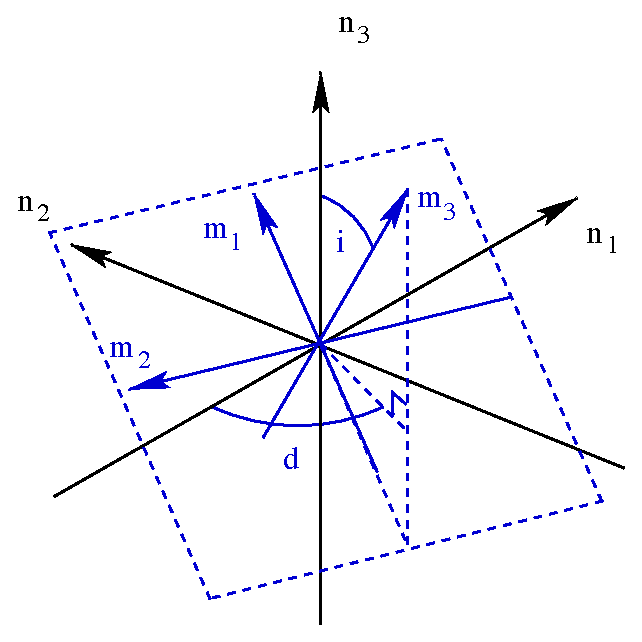
\includegraphics[width=6cm]{figs/figure3.eps}
      \caption{The dial face.\label{dialGeom}}
    \end{center}
  \end{minipage}
  \hfill
  \begin{minipage}[t]{.45\textwidth}
    \begin{center}  
      \includegraphics[width=6cm]{figs/figure4.eps}
      \caption{The gnomon.\label{gnomonGeom}}
    \end{center}
  \end{minipage}
  \hfill
\end{figure}
%
% ----------------------------------------------------------------- %
\section{The calculation} \label{mainCalc}
%
We can now solve the general sundial problem; given a gnomon with arbitrary orientation, casting a shadow onto a plane, the dial face, also of arbitrary orientation, where does the tip of the shadow lie in relation to the intersection of the gnomon and the dial face?

Lines on a sundial are typically constructed relative to the shadow at noon (the ``noon line''). Noon occurs when the sun passes through the meridian plane $M=n_1 \wdg n_3$. 
Equivalently, we have the condition that $s$ lies in $M$
%
\begin{equation}
s \wdg M = 0
\end{equation}
%
Solving this equation gives the condition
%
\begin{equation} \label{noonCond}
\tan\psi = \frac{ \tan\sigma }{ \cos\alpha }.
\end{equation}
%
At an arbitrary time, the shadow is parallel to the intersection of the planes $G$ and $S$, where $S = s \wdg g$. To find this intersection we first form $G \crs S$; the plane perpendicular to both $G$ and $S$, where $\crs$ denotes the commutator product. The vector we seek is dual to this plane so the shadow is parallel to
%
\begin{equation} \label{shadVec1}
u = I\, G\crs S = \la IGS \ra_1.
\end{equation}
%
The magnitude of $u$ is $\sin \Psi$ where $\Psi$ is the angle between the planes $S$ and $G$. Dividing by this magnitude gives
%
\begin{equation} \label{shadVec}
\what = \frac{1}{\sin\Psi} u,
\end{equation}
%
a unit vector parallel to the shadow. Substituting (\ref{noonCond}) into (\ref{shadVec}) gives us the noon line $\what_{noon}$. We can now compute the angle $\zeta$ between the shadow vector and the noon line
%
\begin{equation} \label{shadBearing}
\cos\zeta = \what \dt \what_{noon}.
\end{equation}
%
We have the azimuthal coordinate of the tip of the shadow in the dial face (relative to the noon line). To obtain the radial coordinate we can construct the vector
%
\begin{equation} \label{shadRadialCoordCond}
w^\prime(\lambda) = g + \lambda s,
\end{equation}
%
which will be equal to the shadow vector $w$ when it lies in the plane of the dial face $G$. (Figure~\ref{shadTriangle}). We therefore impose the condition
%
\begin{equation}
w^\prime(\lambda) \wdg G = 0.
\end{equation}
%
Solving this for $\lambda$, then substituting into (\ref{shadRadialCoordCond}) gives $w$, the shadow itself. Its magnitude $|w|$ is the radial coordinate of the shadow tip. Cartesian coordinates are most naturally expressed relative to the frame of (\ref{mFrame})
%
\begin{equation} \label{cartCoordsShad}
x_i = w \dt m_i \qquad i = 1, 2, 3.
\end{equation}
%
\begin{figure}
\centering
\includegraphics[width=8cm]{figs/figure5.eps}
\caption{The triangle formed in the plane $S$ by the gnomon $g$, the scaled sun-ray vector $\lambda s$ and the shadow $w$ whose length is $L$. The angle between the $g$ and $s$ is $\Xi$ and $\what$ ($w/L$) is obtained by rotating $g$ by the angle $\beta$ in $S$. Also shown (as a dashed line) is the normal projection of $g$ onto the dial face ($G = m_1 \wdg m_2$). This line is not coincident with the shadow, which shows that the angle between the planes $S$ and $G$ is not $90^\circ$; it depends on the geometry and we give it the symbol $\Psi$ (not shown).\label{shadTriangle}}
\end{figure}
%
% ----------------------------------------------------------------- %
\section{Explicit formulae} \label{specCalc}
%
Let us now obtain explicit expressions for the formulae in Section~\ref{mainCalc} for the special case of a gnomon that lies in the meridian plane. Setting $\delta = 0$ in (\ref{gnomon}) gives
%
\begin{equation}
g = \cos\iota \, n_3 - \sin\iota \, n_1.
\end{equation}
%
This leaves enough generality to cover the common types of sundial. In particular, we have a style (gnomon parallel to the Earth's axis) when $\iota = \theta$ and a vertical gnomon when $\iota = 0$. It is useful to define a generalized solar hour angle as the angle between $S$ and $M$ given by
%
\begin{equation} \label{cosmu}
\cos\mu = \frac{-S\cdot M}{\sqrt{-S^2}\sqrt{-M^2}} = \frac{-S\cdot M}{\sin(\Xi)}
\end{equation}
%
where $M^2 = -1$ and $\Xi$, the angle between the direction of sun rays $s$ and the gnomon $g$, is given by
%
\begin{eqnarray}
\cos\Xi & = s\cdot g = & \sin(\iota-\theta)(\cos\sigma\cos\psi\cos\alpha - \sin\sigma\sin\psi) \\ \nn
        && - \cos(\iota-\theta)\cos\sigma\sin\alpha
\end{eqnarray}
%
This gives the magnitude of the bivector $S$ via $S^2 = (s\cdot g)^2 - s^2 g^2 = -\sin^2\Xi$. Evaluating (\ref{cosmu}) gives
\begin{equation} \label{cosHourAngle}
  \cos\mu = \frac{(\sin\psi\sin\sigma+\cos\alpha\cos\psi\cos\sigma)\cos(\iota-\theta)-\sin\alpha\cos\sigma\sin(\iota-\theta)}{\sin\Xi}
\end{equation}  
%
and so
%
\begin{equation} \label{hourAngle}
\tan\mu = \frac{\sin\psi\cos\alpha-\cos\psi\tan\sigma}{( \sin\psi\tan\sigma+\cos\psi\cos\alpha )\cos(\iota-\theta) - \sin\alpha\sin(\iota-\theta) }
\end{equation}
%
In terms of this angle, we can express $S$ in the following simple form
%
\begin{equation} \label{SBetter}
S = -\sin\Xi ( \sin\mu( \sin\iota \, n_1 \wdg n_2 + \cos\iota \, n_2 \wdg n_3 ) - \cos\mu \, n_1 \wdg n_3 )
\end{equation}
%
which, when substituted into (\ref{shadVec1}) gives
%
\begin{eqnarray} \label{shadBetter}
\frac{u}{\sin\Xi} & = & \phantom{-}( \sin\iota\sin d \sin i \sin\mu + \cos i \cos\mu ) \; n_1 \\ \nn
& & - \sin\mu ( \sin\iota\sin i \cos d + \cos\iota\cos i) \; n_2 \\ \nn
& & - \sin i (\cos\iota\sin d \sin\mu - \cos d\cos\mu) \; n_3.
\end{eqnarray}
%
Taking the inner product of this vector with itself yields $\Psi$ where
%
\begin{equation}
\cos\Psi = \sin\mu (\cos i\sin\iota - \sin i\sin\iota\cos d) - \cos\mu \sin i\sin d
\end{equation}
%
which in turn allows us to construct $\what$ via (\ref{shadVec}). To evaluate $\what$ at noon we impose the condition in (\ref{noonCond}) which amounts to setting $\mu = 0$. This yields
%
\begin{equation}
\what_{noon} = \frac{1}{\upsilon(i,d)}(\cos i \; n_1 + \sin i\cos d\; n_2)
\end{equation}
%
where
%
\begin{equation}
\upsilon(i,d) = (\cos^2 i + \sin^2 i\cos^2 d)^{1/2}.
\end{equation}
%
In the above, all of the dependence on $\sigma$, $\psi$ and $\alpha$, the physical parameters of the Earth's orbit is contained within $\mu$ and we have have formulae which relate $\mu$ to the geometry we have chosen for the sundial ($i$, $d$ and $\iota$). Our expression for the shadow angle (\ref{shadBearing}) then yields
%
\begin{equation} \label{tanzeta}
\tan\zeta = \frac{\tan\mu(\sin\iota\sin i \cos d + \cos\iota\cos i)}
{\upsilon^2(i,d) - \tan\mu\sin d\sin i(\sin\iota\cos i - \cos\iota\sin i\cos d)}.
\end{equation}
%
This expression gives the angular coordinate of the tip of the shadow on the face of the dial $G$. To find the length of the shadow, we solve (\ref{shadRadialCoordCond}) for $\lambda$ which gives
%
\begin{equation}
\lambda = \frac{\cos\iota\cos i + \sin\iota\sin i \cos d}{D}
\end{equation}
%
where
%
\begin{eqnarray} \label{D}
D & = & (\sin i \cos d \cos\theta-\sin\theta\cos i)\cos\mu_s-\sin\mu_s \sin d\sin i)\sin\Xi \\ \nn
  &   & +(\sin i\sin\theta\cos d+\cos i\cos\theta)\sin\alpha\cos\sigma
\end{eqnarray}
%
and $\mu_s$ is the hour angle from \ref{hourAngle} subject to the condition $\iota = \theta$ such that $g$ is a style. We can now substitute for $\lambda$ in (\ref{shadRadialCoordCond}) to get the shadow vector $w$ which has magnitude
%
\begin{equation} \label{L}
L = \frac{\sin\Xi\sin\Psi}{D}.
\end{equation}
%
Projecting $w$ onto the frame of (\ref{mFrame}) (as in (\ref{cartCoordsShad})) gives the Cartesian coordinates of the tip of the shadow
%
\begin{eqnarray} \label{shadTipCartCoords}
\frac{x}{L} & = &  \frac{1}{\sin\Psi} (\cos\mu\cos d - \sin\mu\cos\iota\sin d)\\ \nn
\frac{y}{L} & = & \frac{-1}{\sin\Psi} (\sin\mu[\sin\iota\sin i + \cos\iota\cos i\cos d] + \cos\mu\cos i\sin d)\\ \nn
\frac{z}{L} & = & 0.
\end{eqnarray}
%
Substituting for $L$ using \ref{L} and eliminating the hour angle $\mu$ using \ref{cosHourAngle}, we arrive at the following expanded forms for $x$ and $y$.
\begin{eqnarray} \label{shadTipCartCoordsExpanded}
  x & = & \bigg[ (\cos(d)\cos(\iota - \theta)\tan(\sigma) - \sin(d)\cos(\alpha)\cos(\iota))\sin(\psi)\\ \nn
    &   & + (\sin(d)\cos(\iota)\tan(\sigma) + \cos(\alpha)\cos(d)\cos(\iota - \theta))\cos(\psi)\nn \\ \nn
    &   & - \sin(\alpha)\sin(\iota - \theta)\cos(d) \bigg] \frac{1}{D}\\ \nn
  y & = & \bigg[ [(\sin(i)\sin(\iota) + \cos(d)\cos(i)\cos(\iota))\tan(\sigma) - \sin(d)\cos(\alpha)\cos(i)\cos(\iota - \theta)]\cos(\psi)\\ \nn
    &   & - [\sin(d)\cos(i)\cos(\iota - \theta)\tan(\sigma) + \sin(i)\sin(\iota)\cos(\alpha) + \cos(\alpha)\cos(d)\cos(i)\cos(\iota)]\sin(\psi)\\ \nn
    &   & + \sin(\alpha)\sin(\iota - \theta)\sin(d)\cos(i) \bigg] \frac{1}{D}
  \end{eqnarray}
%
where
%
\begin{eqnarray} \label{shadTipCartCoordsDenomExpanded}
  D & = & -(\sin(\psi)\cos(\alpha) - \cos(\psi)\tan(\sigma))\sin(d)\sin(i)\\ \nn
    &   & + (\sin(i)\cos(\theta)\cos(d) - \cos(i)\sin(\theta)) (\cos(\psi)\cos(\alpha) + \sin(\psi)\tan(\sigma))\\ \nn
    &   & + (\sin(i)\sin(\theta)\cos(d) + \cos(i)\cos(\theta))\sin(\alpha)
\end{eqnarray}
%
Finally, let us perform a useful consistency check. We have two ways of finding the angle $\beta$ between $g$ and $w$. One is to use the triangle defined by $g$, $w$ and $\lambda\,s$ and the other is to form the inner product $g \dt \what$. The former entails using the sine rule to evaluate
%
\begin{equation} \label{sinbeta}
\sin\beta = \frac{\lambda\sin\Xi}{L}
\end{equation}
%
and the latter gives
%
\begin{equation}\label{cosbeta}
\cos\beta = g \dt \what.
\end{equation}
%
It can be verified that squaring and adding Equations~\ref{sinbeta} and \ref{cosbeta} does indeed give 1, while the explicit form of $\beta$ is
%
\begin{equation} \label{tanbeta}
\tan\beta = \frac{\sin\iota\sin i\cos d + \cos\iota\cos i}
{\cos\mu( \cos\iota\sin i\cos d - \sin\iota\cos i ) - \sin\mu \sin d \sin i}.
\end{equation}
%
% ----------------------------------------------------------------- %
\section{The equation of time} \label{eot}
%
We have in (\ref{shadTipCartCoords}) (or equivalently Equations~(\ref{tanzeta}) and (\ref{L})) a description of the path of the tip of the shadow as a function of fixed parameters which encode the dial's geometry and the angle $\mu$ which varies with time. $\mu$ is given by (\ref{hourAngle}) as a function of fixed parameters encoding the Earth's orientation, dial's latitude and gnomon's orientation, and the two angles $\sigma$ and $\psi$ which change with time. It is to this time-dependence we now turn. If we restrict to the special case where the gnomon is a style ($\iota = \theta$), $\mu$ becomes the hour angle of the sun
%
\begin{equation} \label{trueHourAngle}
\tan\mu = \frac{\tan\sigma - \tan\psi\cos\alpha}{\tan\sigma\tan\psi + \cos\alpha}
\end{equation}
%
which, if we reduce the tilt of the Earth's axis $\alpha$ to zero, gives $\mu = \sigma - \psi$ as we would expect. $\sigma$ measures the progress of the Earth on its elliptical orbit around the sun which we can express in terms of the semi-major axis $a$, semi-minor axis $b$, eccentricity $e = \sqrt{1 - b^2/a^2}$ and the parameter $\tau$ as
%
\begin{eqnarray} \label{keplerCoords}
\tan\phi(\tau) & = & \frac{b}{a} \frac{\sin \om \tau}{e + \cos \om \tau} \\ \nn
t(\tau) & = & a\left(\tau + \frac{e}{\omega}\sin \om \tau\right).
\end{eqnarray}
%
where $\omega = a\omy$ and $\omy$ is the mean angular frequency of the Earth's orbit ($2\pi$ divided by the time between two successive vernal equinoxes). For a derivation of the above formulae, see Appendix \ref{kepler}. $\phi$ is the angle between the Earth-sun vector $s$ at perihelion and $s$ at an arbitrary time $t$. We assume that $e$ is constant, when in fact it varies slightly with a period of $\sim 10^5$ years -- by allowing $e$ to become a function of time we could model this behaviour. In addition, we are free to choose orbital parameters corresponding to any planet in the solar system, but here we focus on the Earth. The ellipse of the Earth's orbit is rotated by an angle $\rho$ relative to the $\{e_i\}$ frame which is aligned with the equinoxes and solstices (at present $\rho \sim 12.25^\circ$) and perihelion is closest to $-e_1$. The angle $\sigma$ is therefore related to $\phi$ by
%
\begin{equation}
\sigma = \rho + \pi + \phi.
\end{equation}
%
The angle $\psi$ measures the rate at which the Earth spins on its axis, relative to the fixed stars. When $\psi$ increases by $2\pi$, one siderial day ($T_{sd}$) will have elapsed on Earth. We therefore have
%
\begin{equation} \label{psi1}
\psi = \omsd\, t, \qquad \omsd = \frac{2\pi}{T_{sd}}.
\end{equation}
%
Let $N$ be the number of mean days in a year ($T_y$). Note that $N$ is not an integer and is approximately equal to 365.2422. The number of siderial days in $T_y$ is $N+1$, so we can express $\psi$ as
%
\begin{equation}
\psi = \frac{N+1}{N}\omd\,t
\end{equation}
%
where
%
\begin{equation}
\omd = \frac{2\pi}{T_d} \quad \mathrm{and} \quad T_d = \frac{T_y}{N}.
\end{equation}
%
Given the above, (\ref{trueHourAngle}) gives the hour angle of the sun as a function of time. This hour angle is zero at solar noon, but this does not correspond to 12 o'clock as read on mechanical clocks. The latter time is called mean time and increases linearly with absolute, Newtonian time. Solar time is sometimes called true time, but I find this misleading as mean time is much closer to what we mean by ``time''. Solar time varies according to (\ref{trueHourAngle}), as the angle between $s$ and the Earth's axis ($f_3$) changes and as the angular speed of the Earth changes throughout its orbit.

The difference between solar time and mean time is called the equation of time which we shall denote by $\Delta\mu$. To calculate it, we first need an expression for the hour angle of the mean sun. This is the sun as observed on an Earth whose axis is not tilted ($\alpha = 0$) and whose orbit is circular with period $T_y$. In this scenario, we have
%
\begin{equation} \label{meanHourAngle}
\mu_m = \psi + \pi - \sigma.
\end{equation}
%
This mean Earth still spins at the same rate $\omsd$ so the expression for $\psi$ is unaltered from (\ref{psi1}), but now $\sigma$ also goes linearly with time; $\sigma = \omy t $. If we start our clock at perihelion ($t_p$), then $\psi$ and $\sigma$ are given by
%
\begin{eqnarray}
\psi & = & \rho + \omsd (t - t_p) \\ \nn
\sigma & = & \rho + \pi + \omy (t - t_p)
\end{eqnarray}
%
which, upon substituting into (\ref{meanHourAngle}) gives
%
\begin{equation}
\mu_m = \omd (t - t_p).
\end{equation}
%
Mean noon occurs when this angle is equal to $2\pi n$ where $n=0,1,2..$. This occurs at time $t_{mn}$ given by
%
\begin{equation}
t_{mn} = t_p + n T_d.
\end{equation}
%
Figure~\ref{EOT} shows $\Delta_\mu = \mu - \mu_m$ as given by Equations~\ref{trueHourAngle} and \ref{meanHourAngle}. It also shows the two separate effects contributing to $\Delta_\mu$; non-zero $\alpha$ and the non-constant angular speed of a Keplerian orbit. The result for $\Delta_\mu$ in this section is exact and requires a numerical root-finding calculation to find $\tau(t)$ from (\ref{keplerCoords}). However, the fact that $\Delta_\mu$ is composed of the sum of two functions with a high degree of periodicity means that a Fourier series with just two terms provides a very good approximation. Such an expansion is derived in \cite{mueller}\footnote{Also available online at\\ {\tt http://info.ifpan.edu.pl/firststep/aw-works/fsII/mul/mueller.html}}.
%
\begin{figure}[ht!]
\centering
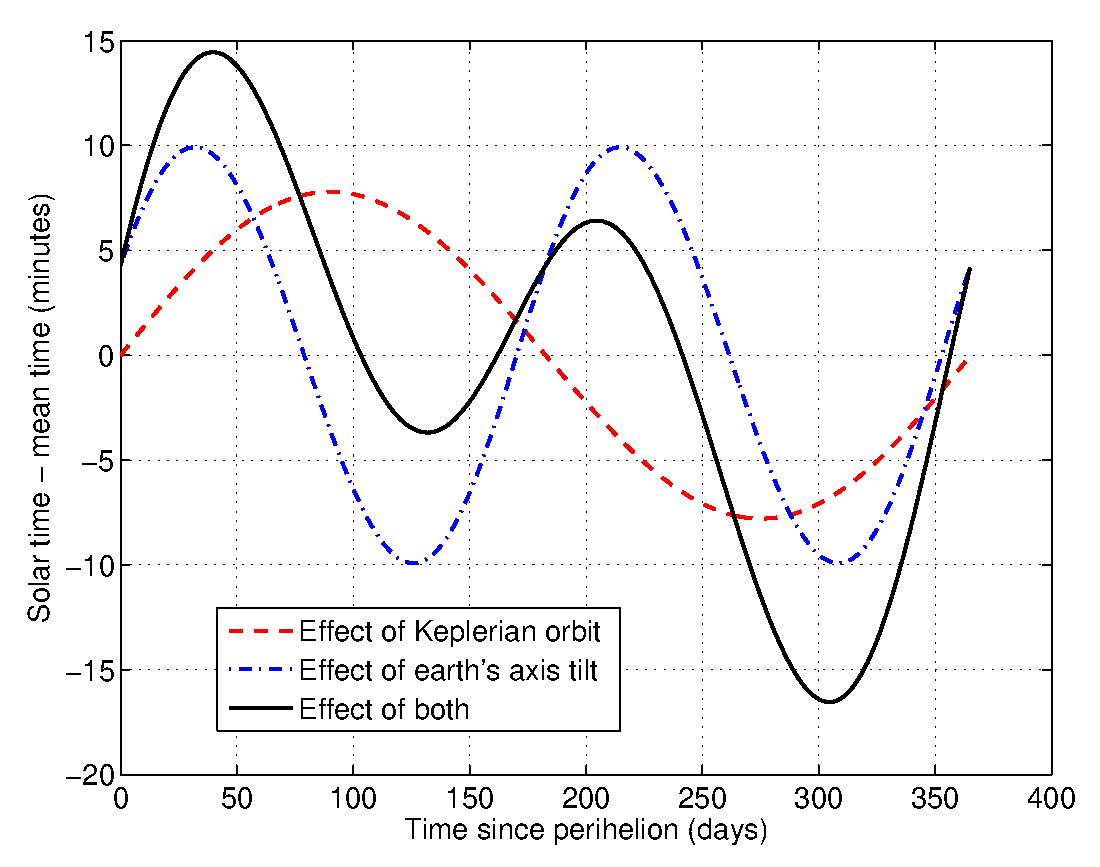
\includegraphics[width=13cm]{figs/figure6.eps}
\caption{The equation of time -- the difference between time as reckoned by the observed hour angle of the sun and the hour angle of an imaginary mean sun. The latter time is ``true'', absolute Newtonian time, the time told by mechanical clocks.\label{EOT}}
\end{figure}
%
% ----------------------------------------------------------------- %
\section{Example paths of the shadow tip} \label{secPaths}
%
The results of Section~\ref{eot} have provided us with a means of plotting the shadow tip's locus at any point in time. In this section we will plot this path for some different dial geometries and locations. Throughout, we will consider a dial on Earth for which $\alpha = 23.5^\circ$. In Figure~\ref{horizDial} we have a horizontal dial where the inclination and declination are both zero ($i = d = 0$) and where the gnomon is a style with $\iota = \theta$. Distances are shown in units of the length of the style whose base is shown by a small circle at the origin of the coordinate system and an embedded compass indicates orientation. The compass diagram results from a vertical projection of a horizontal compass onto the dial face.
%
\begin{figure}[ht!]
\centering
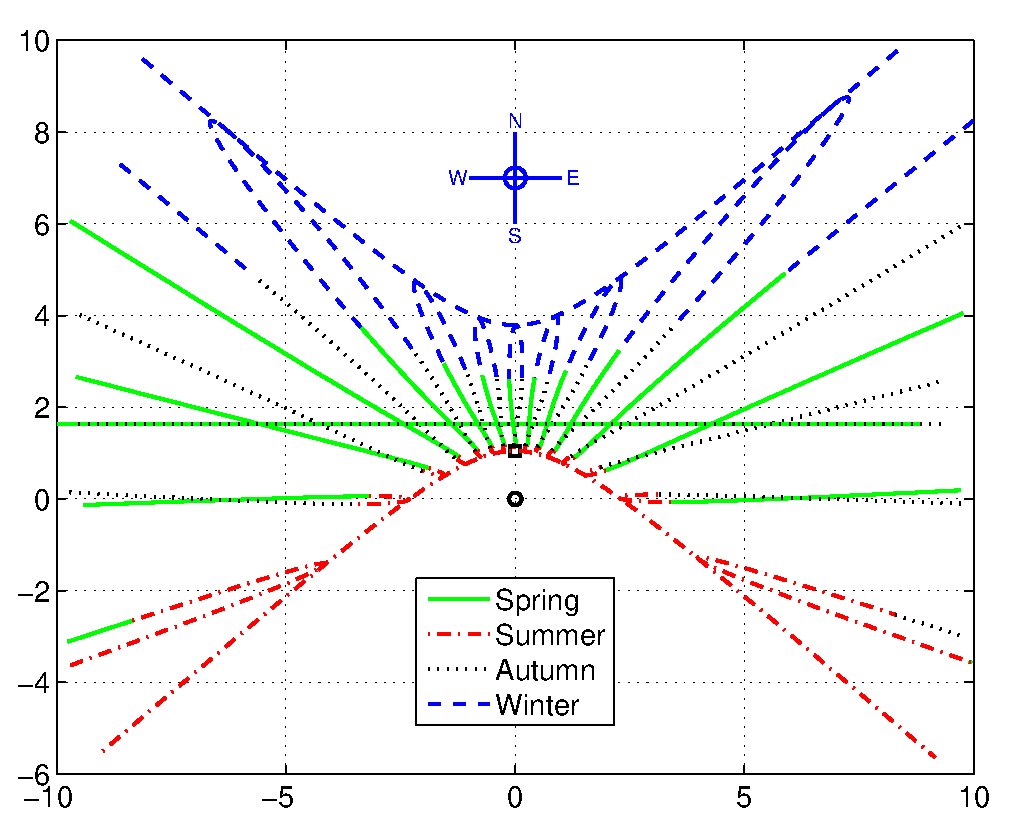
\includegraphics[width=13cm]{figs/figure7.eps}
\caption{The path of the tip of a style's shadow on a horizontal dial face, located at the latitude of Cambridge, England at different times of day and times of year. The characteristic double loop of the analemma is visible at each hour (12 o'clock is marked by a small square). Different times of year are shown with different line styles. The style is of unit length and its base is shown as a small circle. Also shown is the path of the shadow tip on four important days of the year; the equinoxes and solstices. The two paths at the equinoxes coincide while those at the solstices mark the upper and lower limits of the shadow.\label{horizDial}}
\end{figure}
%
The path of the shadow tip for a given time of day as a function of time of year is visible as a figure-of-eight pattern (called an analemma), though in this figure, one side of the double loop is barely visible. A small square marks the 12 o'clock loop. Also shown is the path of the shadow tip as a function of time of day on four key days of the year; the solstices and equinoxes. Points falling in the four seasons are shown in different line styles so we can see, for example, that at the winter solstice the shadow tip passes furthest from the base of the gnomon while at the summer solstice it reaches its closest point. We can see that at both the vernal and autumnal equinoxes the shadow tip passes over the same straight line on the dial face. Near noon, the whole loop for each hour is visible in the figure but for late and early times there is only room to show the summer part of the loop. Seasons are here defined to be 3 month periods of time centered on the solstices and equinoxes and so differ from the seasons we use on the common calendar.

We are of course free to choose an arbitrary dial geometry. Figure~\ref{arbDial} shows the same plot but for a latitude of $10^\circ$ S $(\theta = 100^\circ)$ and dial parameters $i = 15^\circ$, $d = 20^\circ$ and $\iota = 20^\circ$.The proximity of the dial to the equator gives a only small variation between shadow length between winter and summer, as we would expect.
%
\begin{figure}[ht!]
\centering
\includegraphics[width=13cm]{figs/figure8.eps} 
\caption{Paths of the shadow tip for a dial near the equator in the Southern hemisphere (latitude $10^\circ$ South) with an unusual geometry; inclination $i = 15^\circ$, declination $d = 20^\circ$ and gnomon angle $\iota = 20^\circ$.\label{arbDial}}
\end{figure}
%
In plotting these shadow paths it is useful to know the times of sunrise and sun set. These events occur when the shadow length $L$ becomes infinite. It is sufficient to examine the zeros of $D$ -- taking the horizontal dial as an example, $D$ becomes
%
\begin{equation} \label{D_h}
D_h = \cos\theta\sin\alpha\cos\sigma - \sin\theta( \cos\alpha\cos\psi\cos\sigma - \sin\psi\sin\sigma).
\end{equation}
%
Setting this equal to zero yields a quadratic equation for $\sin\psi$ whose solutions give the time of day of sunrise and sunset. The discriminant of this equation is greater than zero when
%
\begin{equation} \label{tantheta_crit}
\tan\theta > \frac{\sin\alpha}{(\tan^2\sigma + \cos^2\alpha)^{1/2}} \quad ( = \tan\mathcal{D})
\end{equation}
%
which gives a condition on the latitude for a sunset and sunrise to exist. At the summer solstice when $\sigma = 0$ we can see that (\ref{tantheta_crit}) reduces to $\theta > \alpha$ so that the sun rises and sets only if we are outside the arctic circle. At the equinoxes when $\sigma = \pi/2$ and $3\pi/2$ we have $\theta = 0$ and $\pi$, corresponding a sunrise and sunset occurring over the entire planet. At the poles themselves, this occurs for a unique value of $\sigma$, giving only one sunrise and one sunset per year. The right hand side of (\ref{tantheta_crit}) is just the (tangent of the) declination of the sun $\mathcal{D}$; the angle between the vector $s$ and the equatorial plane $f_1 \wdg f_2$.

To calculate the hours at which the analemma is first and last visible on a dial face of arbitrary orientation, we must perform a similar calculation to the above but now for the general form of $D$ given by (\ref{D}). In this case, it is simplest to proceed numerically and this approach was taken for the figures in this section. Figure~\ref{articDial} shows a dial in the arctic for which, during the height of summer, the sun does not set. During the spring and autumn, we do have a sunset and sunrise.
%
\begin{figure}[ht!]
\centering
\includegraphics[width=13cm]{figs/figure9.eps} 
\caption{Paths of the shadow tip for a dial in the arctic (latitude $80^\circ$ North) and with a declination of $d = 30^\circ$. The gnomon here is a true gnomon, being vertical, with $\iota = 0^\circ$.\label{articDial}}
\end{figure}
%
% ----------------------------------------------------------------- %
\section{Comparison with existing results}\label{secComparison}
%
The problem of calculating the angle made by the shadow of a gnomon is among the oldest in geometry so it is no surprise that there is an established literature on the subject. My main reference here will be \cite{Rohr} which records results for standard types of sundial, but \cite{waugh} also has some useful information. While Rohr considers an arbitrarily oriented dial face, he uses a style throughout, expect for the case of an analemmatic sundial, where the dial face is horizontal and the gnomon is vertical.

The substyle $b$ is the projection of the style onto the dial face in the direction of its normal. We can obtain a vector parallel to $b$ by rotating $G \dt g$ by $\pi/2$ in $G$ to get
%
\begin{equation}
b = \left(\sin\iota\cos i\cos d - \cos\iota\sin d\right)\,m_1 - \sin\iota\sin d\,m_2.
\end{equation}
%
The length of this vector is the cosine of the angle $A$ between $g$ and $b$
where
%
\begin{equation}
\sin A = \sin\iota\sin i\cos d + \cos\iota\cos i.
\end{equation}
%
The angle between the substyle and the noon line $B$ is given by
%
\begin{equation}
\cos B = \frac{1}{|b|} b \dt w_{noon}
\end{equation}
%
which yields
%
\begin{equation}
\tan B = \frac{\sin i\sin d \left( \tan i\tan\iota\cos d + 1 \right)}{\tan i\cos d - \tan\iota}
\end{equation}
%
For the case considered by Rohr, $\iota = \pi/2 - \theta_L$ and we have
%
\begin{equation}
\tan B = \frac{\sin i\sin d \left( \tan i\cos d + \tan\theta_L \right)}{\tan i\cos d\tan\theta_L - 1}
\end{equation}
%
which agrees with Rohr.
%
% ----------------------------------------------------------------- %
\subsection{Common types of sundial} \label{secCommonTypes}
%
We now focus attention of a selection of special cases of the formulae given in Section~\ref{mainCalc} which corresponds to common types of sundial and show that the results agree with standard formulae.
%
\subsubsection*{Equatorial.}
%
We first set $\iota$ to be $\theta$, making the gnomon parallel to the Earth's axis of rotation and thus a style. Setting $i = \theta$ and $d$ to zero gives a dial face parallel to the equatorial plane. The shadow angle (\ref{tanzeta}) reduces to $\mu$, the hour angle (\ref{trueHourAngle}) and the shadow's length becomes
%
\begin{equation}
L = \frac{ \sqrt{\tan^2\sigma + \cos^2\alpha} }{\sin\alpha} = (\tan\mathcal{D})^{-1}
\end{equation}
%
where $\mathcal{D}$ is the sun's declination (\ref{tantheta_crit}).
%
\subsubsection*{Horizontal.}
%
If we instead set both $i$ and $d$ to zero we have a horizontal dial face (tangent to the Earth's surface). The shadow angle (\ref{tanzeta}) becomes
%
\begin{equation}
\tan\zeta = \cos\theta\tan\mu
\end{equation}
%
and the length of the shadow cast by a gnomon of unit length is given by
%
\begin{equation}
L = \frac{\cos\mu}{D_h\tan\mathcal{D}}\sqrt{1 + \tan^2\mu\cos^2\theta}
\end{equation}
%
where $D_h$ is given by (\ref{D_h}).
%
\subsubsection*{Vertical.}
%
If we instead set $i$ to be $\pi/2$ we have a vertical dial where
%
\begin{equation}
\tan\zeta = \sin\theta\tan\mu
\end{equation}
%
\subsubsection*{Inclining.}
%
The vertical dial faces South. If we rotate the dial face about the East-West line, we have an inclining dial. In our formulae, this amounts to allowing $i$ to be arbitrary but fixing $d$ to be zero:
%
\begin{equation}
\tan\zeta = \cos(i-\theta)\tan\mu
\end{equation}
%
%
\subsubsection*{Declining.}
%
If we take a vertical dial and remove the restriction that it faces South, we have a declining dial. This corresponds to $i=\pi/2$ and arbitrary $d$
%
\begin{equation}
\tan\zeta = \frac{\sin\theta\sin\mu}{\cos d\cos\mu + \sin d\sin\mu\cos\theta}
\end{equation}
%
%
\subsubsection*{Both declining and inclining.}
%
Leaving $i$ and $d$ arbitrary, but setting $\iota = \theta$ such that the gnomon is a style, amounts to a simple substitution of $\theta$ for $\iota$ in Equations~\ref{tanzeta} and \ref{L}.
%
% ----------------------------------------------------------------- %
\section{Conclusion}\label{secConclusion}
%
I have presented a different approach to solving the generalized sundial problem where both gnomon and dial face can have arbitrary orientation. This is a more general geometry than that commonly considered in the literature. The calculation placed equal emphasis on both the geometry of the dial and the physics behind the equation of time. For the special case of a gnomon lying in the meridian plane we have explicit formulae for the coordinates of the shadow tip as a function of time. Visualization confirms that the results are consistent with intuition and display familiar features such as the analemma. Finally, I demonstrated that the formulae reduce to known results in special cases corresponding to common types of dial.

It is unlikely that the general results presented here will be used to construct a sundial; construction and usage of sundials is simplest for the special cases considered in Section~\ref{secCommonTypes}. Rather, they may be of more academic interest to sundial enthusiasts. In addition, I hope that this calculation provides a concrete example of the utility of geometric algebra and shows how it can bring power and simplicity to calculations in physics.
%
% ----------------------------------------------------------------- %
\section{Personal note}
%
Toward the end of a visit to see my family in Canada in the summer of 2005, I was sitting with my 93 year-old grandfather in his garden before leaving for the airport at 5pm. I didn't want to be late but had left my watch inside -- I was about to get it to check the time when my grandfather told me not to worry; he had observed that the shadow cast by a fence post was parallel to the sides of the paving slabs of his patio at 5pm the previous day. As the shadow was falling about $15^\circ$ from that line, he said that at a rate of about $1^\circ$ every 4 minutes, I had about an hour left.

Inspired by this, I decided to calculate the angle between the paving slabs and fence shadow during my flight (ie the sundial problem), for some fun on the plane. On returning home, I checked my formulae against the standard results in the literature and was surprised to find that I had approached the problem in what seemed to be a different way, and obtained some more general results. For this initial inspiration, I am grateful to my grandfather, Claude Goyder.
%
\section*{Acknowledgements}
%
I am grateful to \href{https://sites.google.com/view/hanswilschut/home}{Hans W. Wilschut} for finding several typos in the original version.
%
\clearpage
%
% ----------------------------------------------------------------- %
\appendix 
\section{Spinor approach to the Kepler problem} \label{kepler}
%
In Section~\ref{eot} we introduced (\ref{keplerCoords}) for the azimuthal coordinate of the Earth on its elliptical orbit. This expression is derived from the approach to the Kepler problem given in \cite{GAbook}. The orbit is parametrized in terms of the spinor $U$, where
%
\begin{equation} \label{spinorx}
x = U e_1 U^\dag
\end{equation}
%
and where $x$ is the position vector of the Earth's centre of mass relative to that of the orbit's focus. $U$ possesses only even grade elements which, in 3-$d$, means that it is a scalar plus bivector. The bivector encodes the plane of the orbit. $U$ should therefore remind us of a complex number and the above form is reminiscent of the exponential form of a complex number ($x = re^{i\theta}$) which rotates the number 1 in the complex plane by $\theta$ and dilates by $r$. However, it is only when the complex number is split into two and the double-sided rotation law in (\ref{spinorx}) is used that we get a form that generalizes to $n$ dimensions.

Differentiating with respect to time and using the parameter $\tau$ where
%
\begin{equation} \label{dtdtau}
\frac{dt}{d\tau} = r
\end{equation}
%
and
%
\begin{equation}
r = UU^\dag
\end{equation}
%
gives an equation of motion for $U$
%
\begin{equation} \label{Udotdot}
\frac{d^2U}{d\tau^2} = \left(-\frac{kx}{\mu r^2} + \frac{\dot{x}^2}{2} \right) U = -\om^2 U
\end{equation}
%
where
%
\begin{equation}
\om^2 = -\frac{E}{2\mu}
\end{equation}
%
and
%
\begin{equation}
E = \half \mu \dot{x}^2 - \frac{k}{r}.
\end{equation}
%
We have assumed that we are moving in a Newtonian force field where
%
\begin{equation}
\mu \ddot{x} = -\frac{k x}{r^3}.
\end{equation}
%
Equation~(\ref{Udotdot}) is just the SHM equation for $U$ with solution
%
\begin{equation}
U(\tau) = A \exp({\hat{L}\om\tau}) + B \exp({-\hat{L}\om\tau})
\end{equation}
%
where $\hat{L}$ is the unit bivector encoding the plane of the orbit, in this case $e_1 \wdg e_2$. Substituting this form of $U$ into (\ref{spinorx}) gives
%
\begin{equation}
x = \left[ (A^2+B^2)\cos2\om\tau + 2AB \right] \,e_1 + (A^2-B^2)\sin2\om\tau \,e_2
\end{equation}
%
from which we can derive expressions for the radial and azimuthal coordinates of the orbit
%
\begin{eqnarray}
r(\tau) & = & A^2 + B^2 + 2AB\cos2\om\tau \\ \nn
\tan \phi(\tau) & = & \frac{(A^2-B^2)\sin2\om\tau}{(A^2+B^2)\cos2\om\tau + 2AB}.
\end{eqnarray}
%
Integrating (\ref{dtdtau}) then yields
%
\begin{equation}
t(\tau) = (A^2+B^2)\tau + \frac{AB}{\om}\sin2\om\tau
\end{equation}
%
This equation in transcendental in $\tau$ so we cannot obtain a closed form solution for $x(t)$ but we have reduced a problem commonly thought to be one of numerical integration to one of root-finding instead.

The constants $A$ and $B$ are related to the semi-major and minor axes of the ellipse ($a$ and $b$) as follows
%
\begin{eqnarray}
a & = & A^2 + B^2 \\ \nn
b & = & A^2 - B^2
\end{eqnarray}
%
and to the eccentricity $e$ and semi-latus rectum $l$ via
%
\begin{eqnarray}
e & = & \frac{-2AB}{A^2+B^2} \\ \nn
l & = & \frac{(A^2-B^2)^2}{A^2+B^2}
\end{eqnarray}
%
% ----------------------------------------------------------------- %
\begin{thebibliography}{10}
%
\bibitem[Doran and Lasenby 2003]{GAbook}
  Doran~C~J~L and Lasenby~A~N 2003 \textit{Geometric Algebra for Physicists} (Cambridge: Cambridge	University Press)
%
\bibitem[Gull et al 1993]{inanr}
	Gull~S~F, Lasenby~A~N and Doran~C~J~L 1993 \textit{Found. Phys.} {\bf 23}(9), 1175--1201
%
\bibitem[Lasenby et al 2000]{umlfpae}
	 Lasenby~J, Lasenby~A~N and Doran~C~J~L 2000 \textit{Phil. Trans. R. Soc. Lond. A} {\bf 358}, 21--39
%
\bibitem[M\"{u}ller 1995]{mueller}
	M\"{u}ller~M 1995 \textit{Acta Phys. Pol. A} {\bf 88} Supplement, S-49
%
\bibitem[Rohr 1996]{Rohr}
  Rohr~R~R~J 1996 \textit{SUNDIALS History, Theory and Practice} (Mineola, NY: Dover Publications, Inc.)
%
\bibitem[Waugh 1973]{waugh}
  Waugh~A~E 1973 \textit{SUNDIALS Their theory and construction} (New York, NY: Dover Publications, Inc.)
%
\end{thebibliography}
%
\end{document}

